\chapter{Introduction}
    
\fcolorbox{black}[HTML]{E9F0E9}{\parbox{\textwidth}{%
\noindent \textbf{Learning goals}\\
The junior-colleague
\begin{enumerate}[nolistsep]
\item can describe what Spring is
\item can describe what Spring Boot is
\item can explain what a three-tier application is
\item can identify the three layers in a Spring Boot application
\item can explain the responsibilities of the layers in a Spring Boot application
\item can explain the architecture of a Spring RESTful web application
\item can explain what a DTO is
\item can explain what an entity-object is
\item can explain what dependency injection is
\item can explain what a Spring bean is
\item can explain what a Spring container is
\item can explain what a Spring Boot starter is
\end{enumerate}}}


\section{Enterprise Applications with Java}

Spring Boot is een framework om enterprise applications te bouwen met Java.
Enterprise applicaties zijn applicaties die bedrijven bouwen of laten bouwen voor hun klanten en medewerkers.  Enterprise applicaties worden ontwikkeld om de bedrijfsprocessen te ondersteunen. 

Enterprise applicaties hebben specifieke kenmerken. Deze kenmerken komen voort uit de complexe aard en specifieke eisen van grootschalige bedrijfssystemen.  Enkele belangrijke kenmerken van enterprise applicaties vanuit het oogpunt van een ontwikkelaar:

\begin{itemize}
\item{Schaalbaarheid (scalability):} Enterprise applicaties moeten een groot aantal gebruikers en gegevens aankunnen.  Ontwikkelaars moeten de architectuur van de applicatie zodanig ontwerpen dat schalen mogelijk is om een groeiend aantal gebruikers en datavolumes aan te kunnen.

\item{Betrouwbaarheid en hoge beschikbaarheid:} Van enterprise applicaties wordt verwacht dat ze 24/7 beschikbaar zijn en snelle responstijden hebben.  Ontwikkelaars moeten oplossingen voorzien om problemen en downtime te voorkomen.  Ze moeten de betrouwbare werking van de applicatie kunnen garanderen.

\item{Beveiliging:} Enterprise applicaties verwerken gevoelige bedrijfsgegevens, waaronder financiële informatie, klantgegevens,...   Ontwikkelaars moeten robuuste beveiligingsmaatregelen implementeren,  zoals authenticatie,  autorisatie,  versleuteling van gegevens en audittrails,  om de gegevens te beschermen tegen ongeautoriseerde toegang.

\item{Integratie:} Enterprise applicaties moeten vaak worden geïntegreerd met verschillende bestaande systemen zoals databanken en externe services.  Voorbeelden van externe services zijn bijvoorbeeld betaalsystemen en boekhoudpakketten. Ontwikkelaars moeten zorgen voor een veilige en betrouwbare gegevensuitwisseling tussen verschillende enterprise applicaties. 

\item{Aanpasbaarheid en flexibiliteit:} Enterprise applicaties worden gebruikt door gebruikers uit diverse afdelingen en teams binnen een organisatie, elk met hun eigen unieke workflows en eisen. Ontwikkelaars moeten applicaties bouwen die kunnen worden aangepast en geconfigureerd om aan deze specifieke behoeften te voldoen. 
Enterprise applicaties ondergaan vaak veranderingen en updates op basis van veranderende zakelijke behoeften. Daarnaast veranderen de workflows en eisen van de gebruikers ook. 
Ontwikkelaars moeten verandering effectief beheren door versiebeheer, wijzigingstracering en terugrolmechanismen te implementeren.
Afhankelijk van de sector moeten enterprise applicaties voldoen aan specifieke wettelijke normen die doorheen de tijd kunnen veranderen. 

\item{Lange levenscyclus:} Enterprise applicaties hebben meestal een langere levenscyclus dan andere soorten software.  Ontwikkelaars moeten zorgen voor voortdurend onderhoud,  updates en verbeteringen.

\item{Samenwerking en documentatie:} Aangezien meerdere ontwikkelaars en teams mogelijk werken aan verschillende delen van een enterprise applicatie, zijn duidelijke code-documentatie, versiebeheer en samenwerkingsgerichte ontwikkelingspraktijken essentieel.

\item{Testen en kwaliteitsborging:} Grondig testen is essentieel voor enterprise applicaties om bugs, prestatieproblemen en beveiligingskwetsbaarheden te identificeren en aan te pakken. Ontwikkelaars moeten geautomatiseerd testen, unit testing, integratietesting en gebruikersacceptatietests implementeren.

\item{Gebruikerservaring (UX):} Hoewel functionaliteit cruciaal is, is een positieve gebruikerservaring ook belangrijk voor gebruikersacceptatie en productiviteit. Ontwikkelaars moeten streven naar intuïtieve interfaces en workflows die de tevredenheid van gebruikers vergroten.
\end{itemize}

Over het algemeen vereist de ontwikkeling van enterprise applicaties een uitgebreid begrip van bedrijfsprocessen, technische expertise en het vermogen om functionaliteit, prestaties, beveiliging en gebruikerservaring in evenwicht te brengen om te voldoen aan de unieke behoeften van grote organisaties.

In 1999 besliste Sun Microsystems om de programmeertaal Java uit te bereiden om het ontwikkelen van enterprise applicaties te vergemakkelijken.  Met de lancering van J2EE (Java 2 Enterprise Editie) en de applicatie servers om de J2EE-toepassingen op te deployen onstond een schaalbaar en betrouwbaar platform. 
J2EE,  dat wordt hernoemd naar Java EE (Java Platform, Enterprise Edition), verwijst naar een verzameling specificaties. Het bestaat uit een reeks standaarden en API's die ontwikkelaars gebruiken om de enterprise-software te implementeren. 

Wanneer in de tekst wordt verwezen naar "J2EE-specificaties" of "Java EE-specificaties", dan verwijst dit naar de reeks specificaties die Java EE vormen.  Deze specificaties zijn de  beschrijvingen van hoe bepaalde componenten en functionaliteiten in een enterprise Java-applicatie moeten worden geïmplementeerd.  Sun Microsystems en later Oracle, dat in de 2010 Sun Microsystems overneemt, zorgen steeds voor een bruikbare implementatie van hun specificaties. 

In een enterprise applicatie moet het mogelijk zijn om eenvoudig mails te versturen. Daarom werd dus de JavaMail API Design Specificaties uitgeschreven. Dit kan je zien als een uitgebreide analyse van de vereisten.  De Reference implementation is voorzien door Oracle

Yes, besides the JavaMail reference implementation, there are other implementations of the JavaMail API. While the reference implementation is provided by Oracle as part of the Java EE platform, alternative implementations have been developed by various organizations and communities. Some of these implementations include:

Apache Geronimo JavaMail: Apache Geronimo is an open-source application server project that includes its own implementation of the JavaMail API.

IBM WebSphere Application Server JavaMail: IBM's WebSphere Application Server also provides its own implementation of the JavaMail API.

JBoss AS (WildFly) JavaMail: The JBoss Application Server (now known as WildFly) includes its own implementation of the JavaMail API.

Google App Engine JavaMail: Google App Engine provides its own implementation of the JavaMail API tailored for its cloud platform.

Caucho Resin JavaMail: The Resin application server offers its own implementation of the JavaMail API.

These alternative implementations often aim to provide the same functionality as the JavaMail reference implementation while potentially offering additional features or optimizations.  


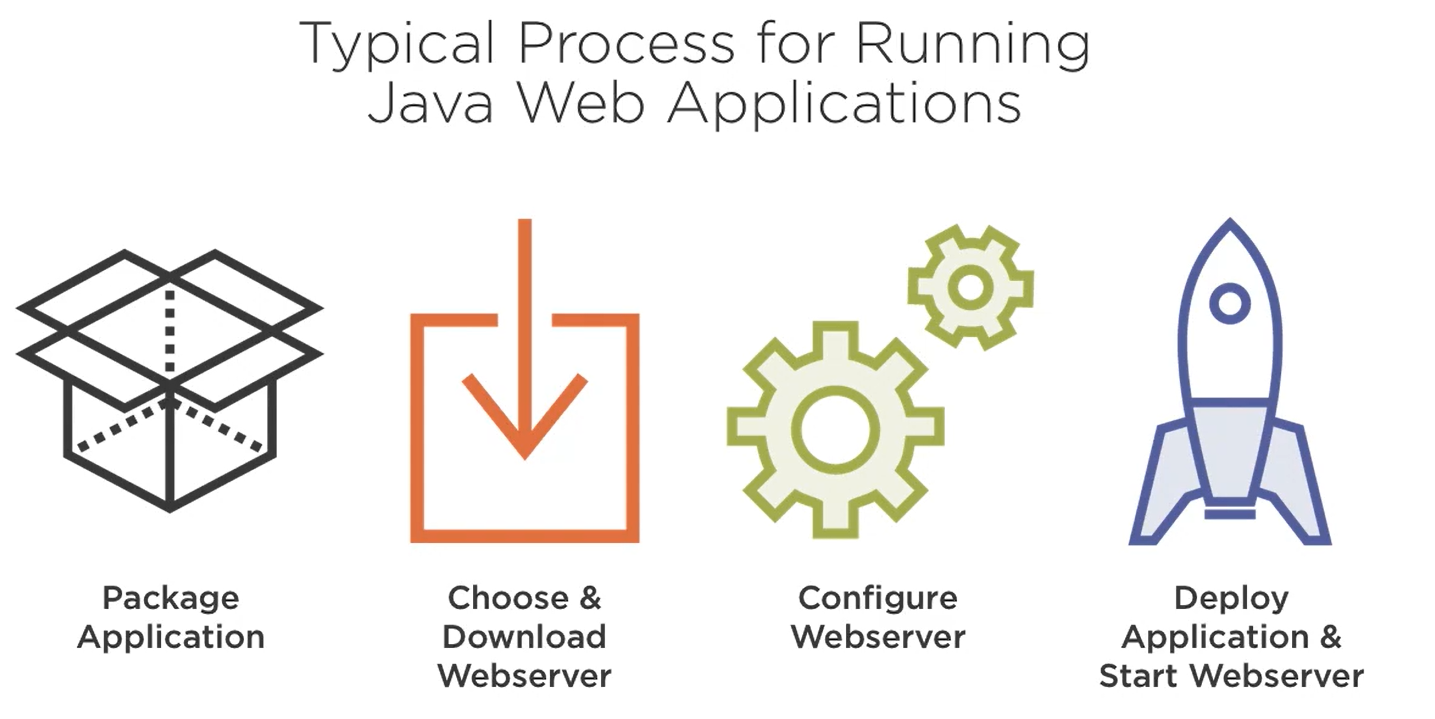
\includegraphics[width=\textwidth]{./images/chapter1/before_spring_boot.png} 

Spring came into being in 2003 as a response to the complexity of the early J2EE specifications. While some consider Java EE and its modern-day successor Jakarta EE to be in competition with Spring, they are in fact complementary. The Spring programming model does not embrace the Jakarta EE platform specification; rather, it integrates with carefully selected individual specifications from the traditional EE umbrella. Spring started as a lightweight alternative to Java Enterprise Edition. Rather than develop components as heavyweight Enterprise
JavaBeans (EJBs), Spring offered a simpler approach to enterprise Java development, utilizing dependency injection and aspect-oriented programming to achieve the capabilities of EJB with plain old Java objects (POJOs).
But while Spring was lightweight in terms of component code, it was heavyweight in terms of configuration. Initially, Spring was configured with XML (and lots of it).
It provides everything you need to create Java enterprise applications. Spring offers the flexibility to create many kinds of architectures depending on an application’s needs. As of Spring Framework 6.0, Spring requires Java 17+.

De lente ontstond in 2003 als reactie op de complexiteit van de vroege J2EE-specificaties. Hoewel sommigen Java EE en zijn moderne opvolger Jakarta EE als concurrenten van Spring beschouwen, zijn ze in feite complementair. Het Spring-programmeringsmodel omarmt niet de Jakarta EE platformspecificatie; in plaats daarvan integreert het met nauwkeurig geselecteerde individuele specificaties uit het traditionele EE-landschap. Spring begon als een lichtgewicht alternatief voor Java Enterprise Edition. In plaats van componenten te ontwikkelen als zware Enterprise JavaBeans (EJB's), bood Spring een eenvoudigere benadering voor enterprise Java-ontwikkeling, waarbij gebruik werd gemaakt van afhankelijkheidsinjectie en aspectgeoriënteerde programmering om de mogelijkheden van EJB te bereiken met gewone Java-objecten (POJO's).
Maar hoewel Spring lichtgewicht was qua componentcode, was het zwaar qua configuratie. In het begin werd Spring geconfigureerd met XML (en veel ervan).
Het biedt alles wat je nodig hebt om Java enterprise-applicaties te maken. Spring biedt de flexibiliteit om verschillende soorten architecturen te creëren, afhankelijk van de behoeften van een applicatie. Vanaf Spring Framework 6.0 vereist Spring Java 17+.

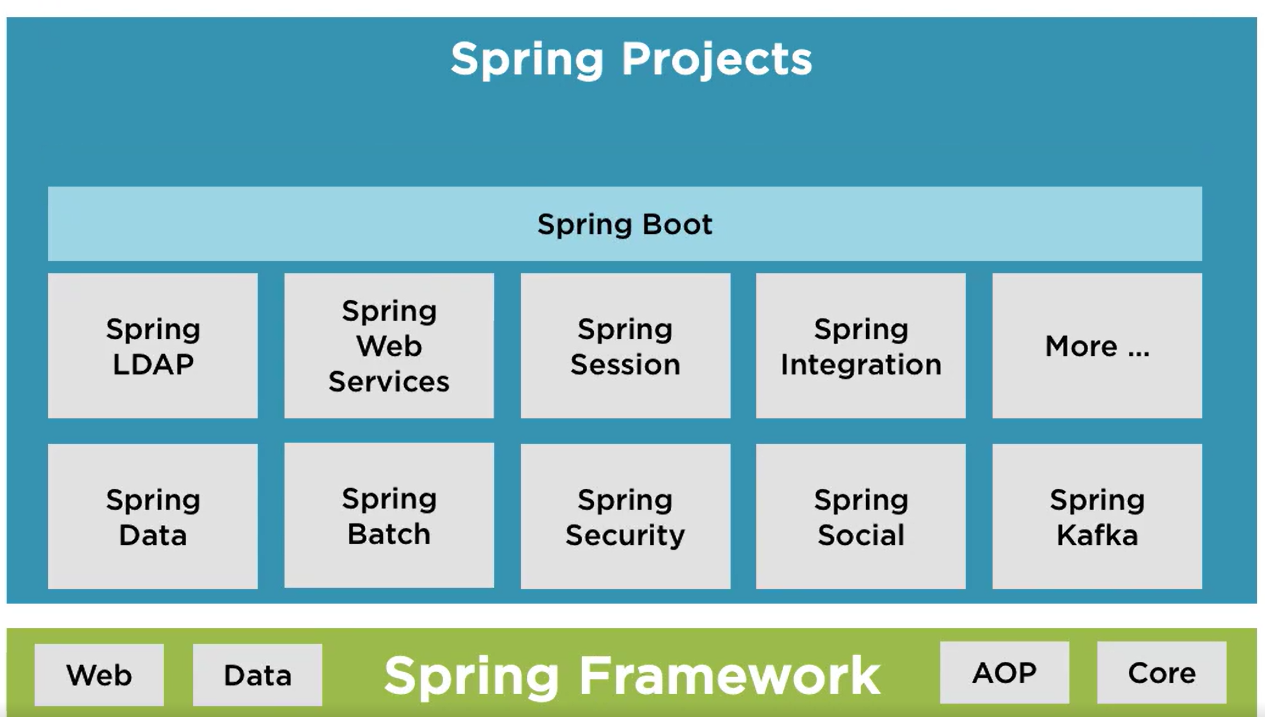
\includegraphics[width=\textwidth]{./images/chapter1/spring_framework.png} 

Spring Boot is a project that is built on the top of the Spring Framework. It provides an easier and faster way to set up, configure, and run java applications.

    
\section{What is Spring Boot?}
 
Spring Boot is an open-source Java framework to create production-ready,  standalone Spring applications. It's a robust, widely used framework. The creation of this framework was facilitated by the desire to simplify the development of applications on the popular Java EE technology stack from Oracle, which was very complex and difficult to use at the time. With very little configuration, you can create easily your first Spring Boot application.

Let's look at some advantages of Spring Boot for developers 
\begin{itemize}
\item speed up the process of creating and deploying application
\item create standalone applications with less or almost no configuration overhead
\item easy to learn framework
\item increase productivity of developers
\end{itemize}

\section{Bootstrapping a simple application}

\subsection{Using Spring Initializr}
Spring Initializr is a web application that can generate a Spring Boot project.
The url for this web application is \url{https://start.spring.io/}. You can select the necessary configuration, including the build tool, language, version of the Spring Boot framework, and any dependencies for your project. IntelliJ IDEA Ultimate provides the Spring Initializr project wizard that integrates with the Spring Initializr API to generate and import your project directly from the IDE.

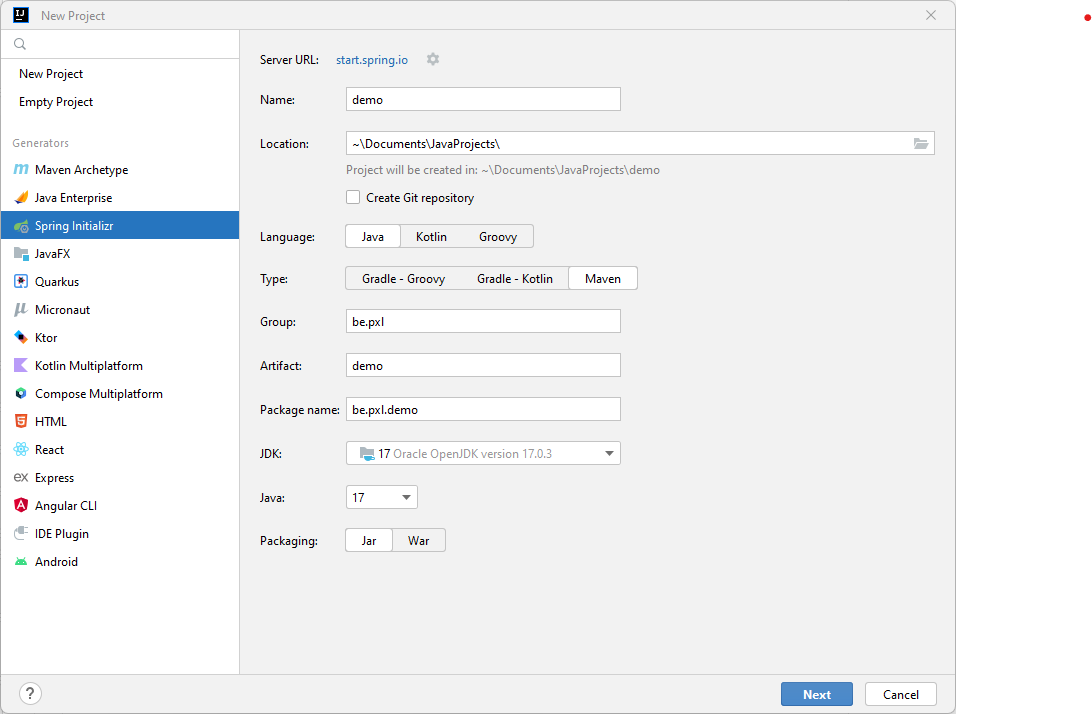
\includegraphics[width=\textwidth]{./images/chapter1/spring_initializer_intellij.png}

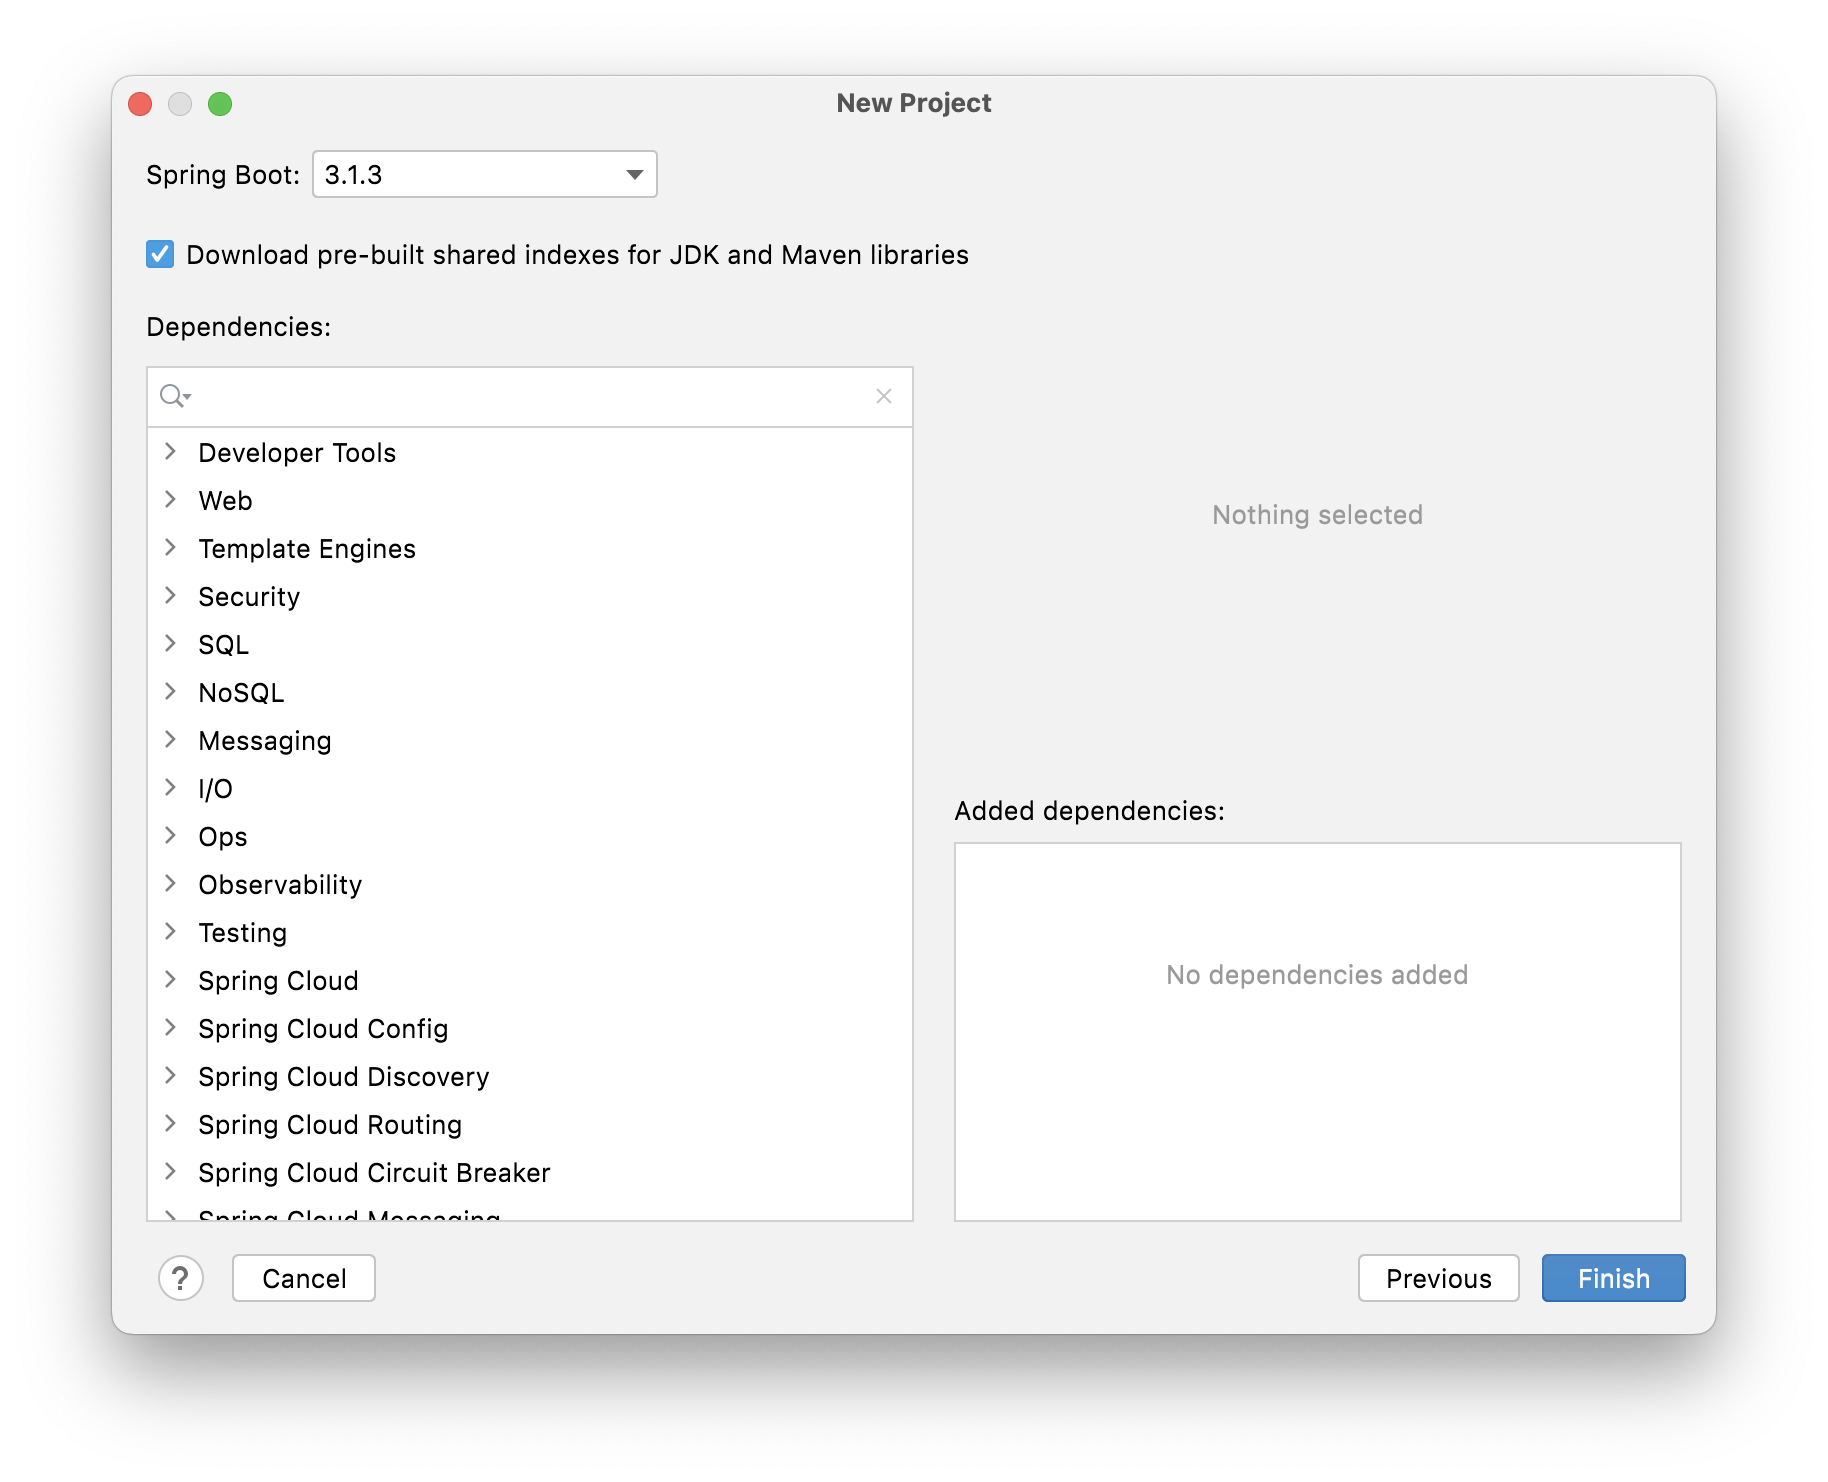
\includegraphics[width=\textwidth]{./images/chapter1/new_project.png}

We select Spring Web dependency. Spring Web uses Spring MVC. It is used for building RESTful Web Services. Spring MVC provides the annotation @RestController for classes that implement the REST endpoints.
To run a RESTful Web Service you need a web container. Spring Boot will automatically add an embedded Tomcat web container to your project. If you prefer another web container, you can update Spring Boot's configuration.
Finally Jackson is a popular third-party library for converting Java-objects to JSON and vice versa.

\begin{oefening}
Create the demo project. You can use the wizard in IntelliJ IDEA Ultimate or \url{https://start.spring.io/}.
\end{oefening}

\section{Running the demo project}

The starting point of a Spring Boot application is the class with the main-method and annotated with @SpringBootApplication.  This class can be found in the folder /src/main/java.  Spring Boot offers a lot of annotations to reduce the workload of developers.   

\begin{lstlisting}[frame=single]
package be.pxl.demo;

import org.springframework.boot.SpringApplication;
import org.springframework.boot.autoconfigure.SpringBootApplication;

@SpringBootApplication
public class DemoApplication {

    public static void main(String[] args) {
        SpringApplication.run(DemoApplication.class, args);
    }

}
\end{lstlisting}

By running the main-class you start your Spring Boot application. 

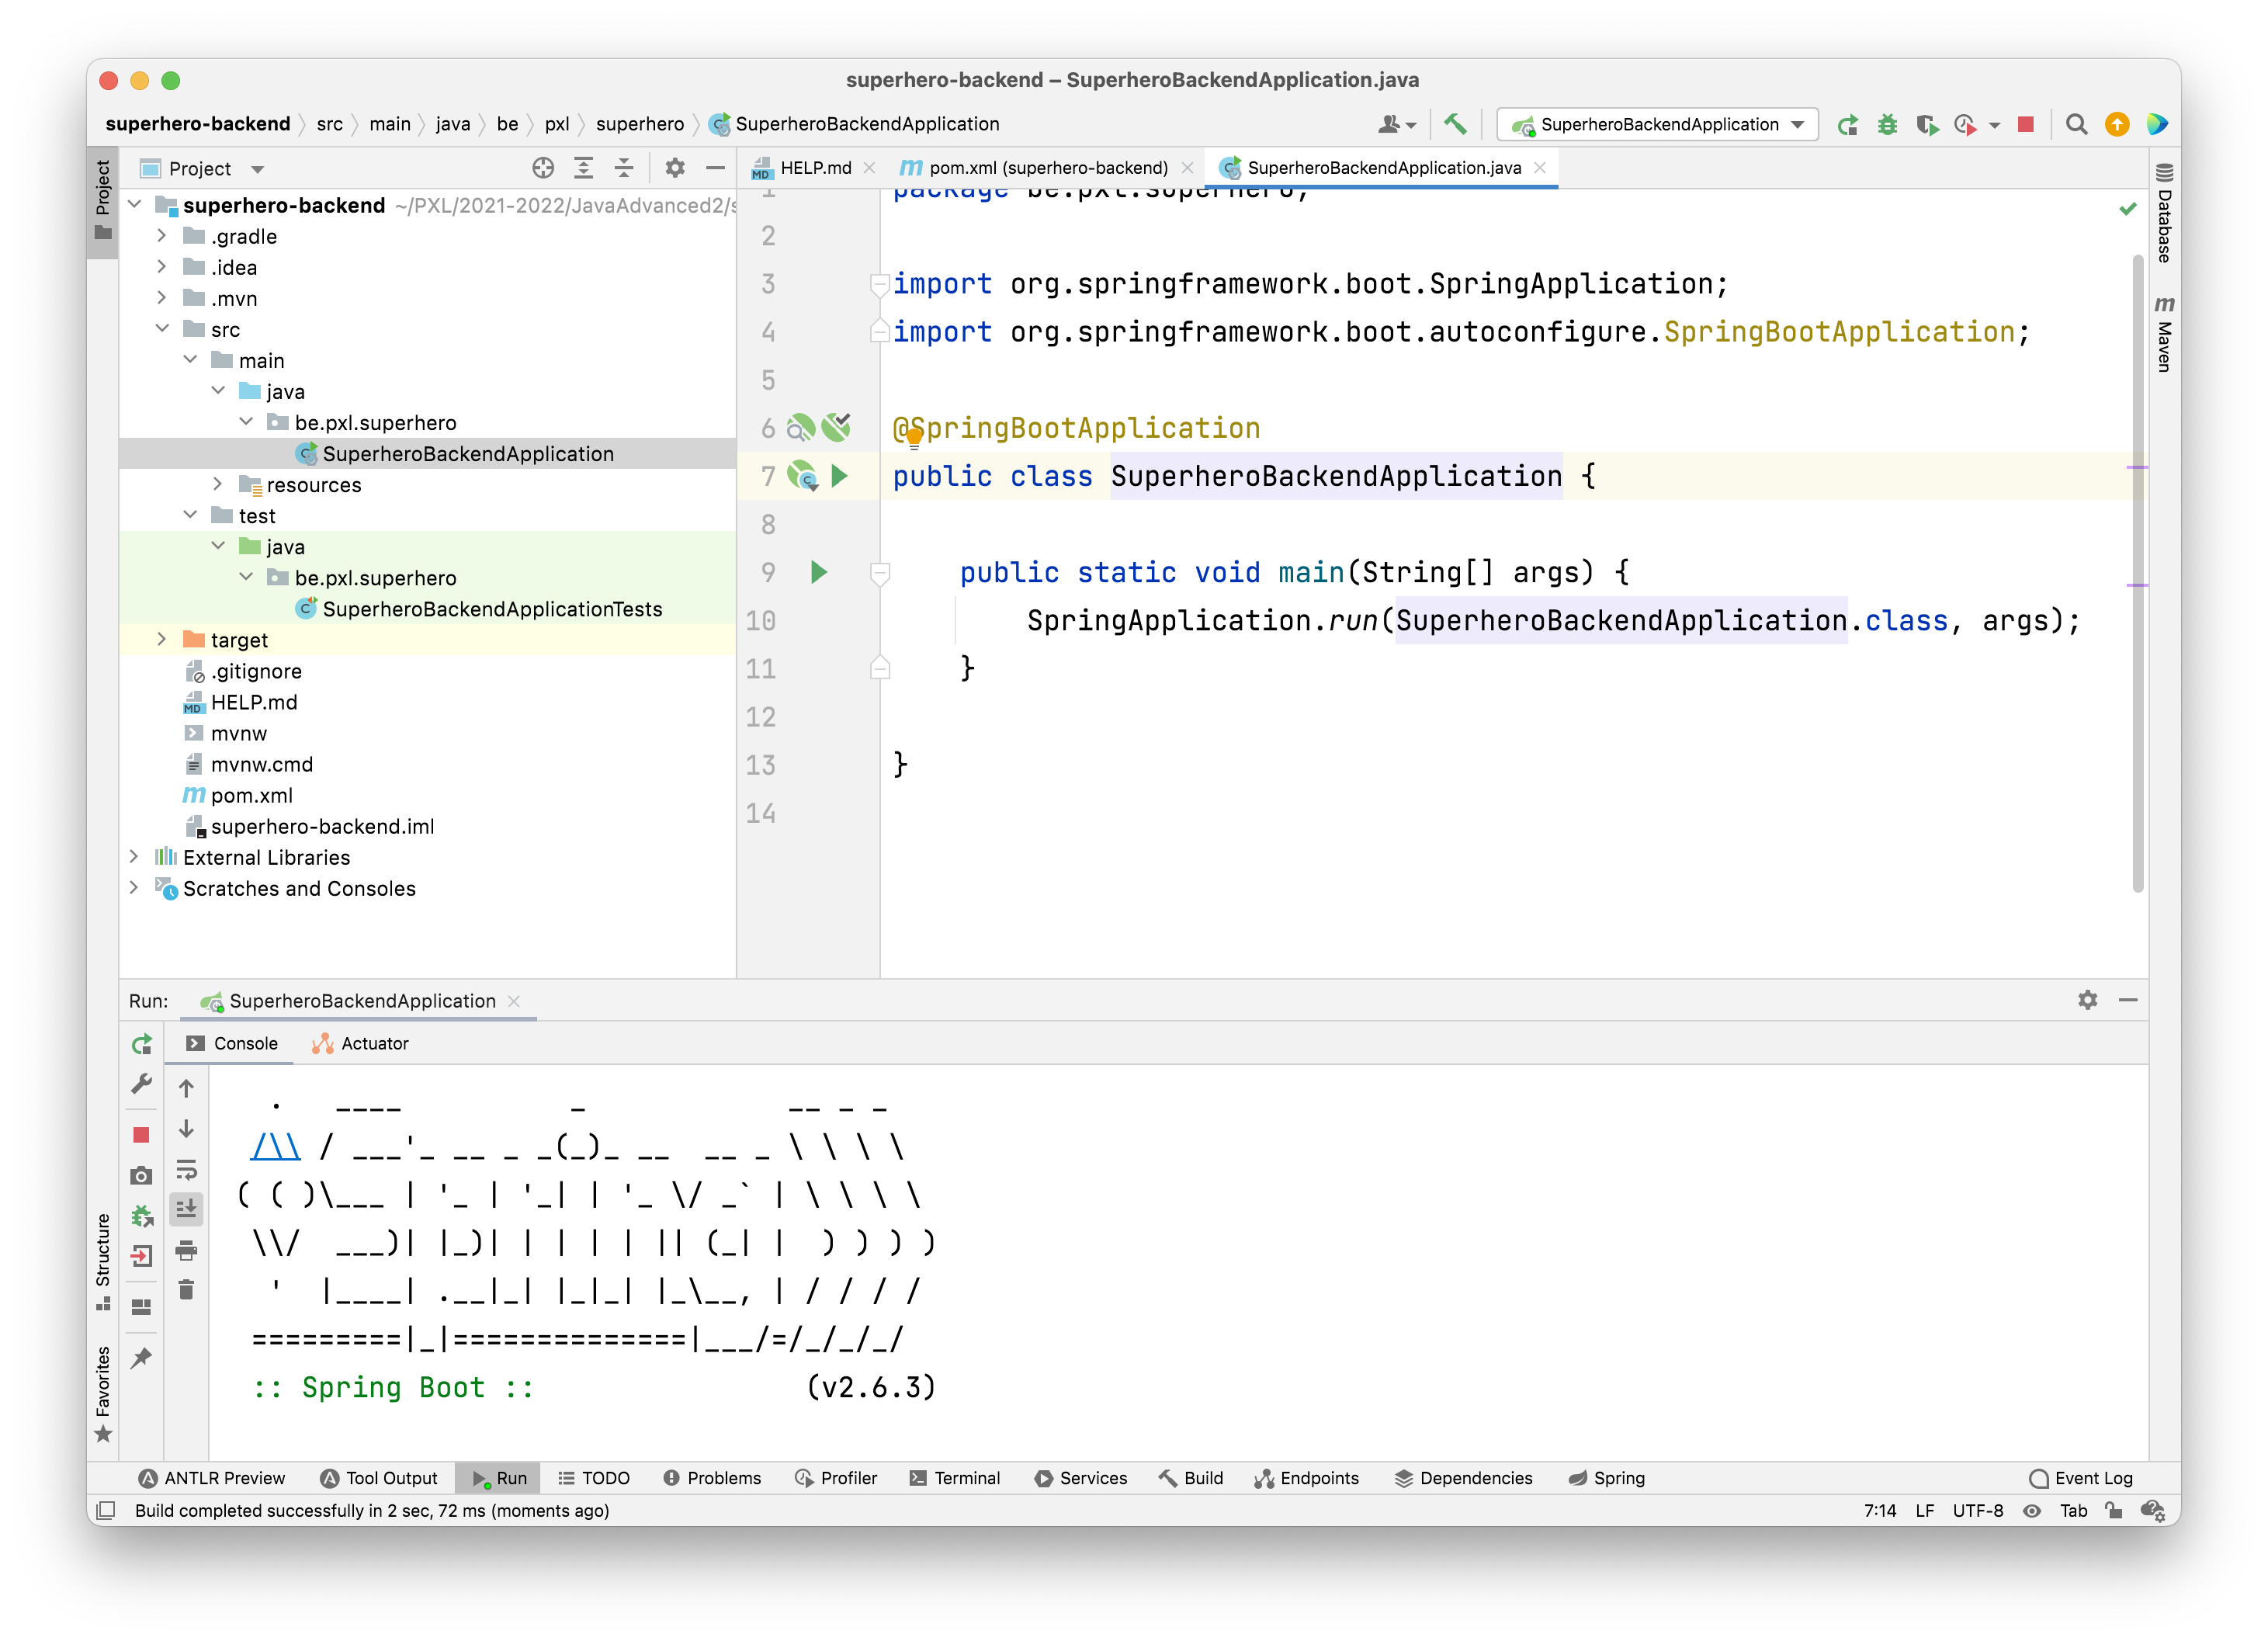
\includegraphics[width=\textwidth]{./images/chapter2/first-run.png}

Currently our Spring Boot application only shows a whitelabel error page. This error page is available when you perform a GET for URL \url{http://localhost:8080}.

\frame{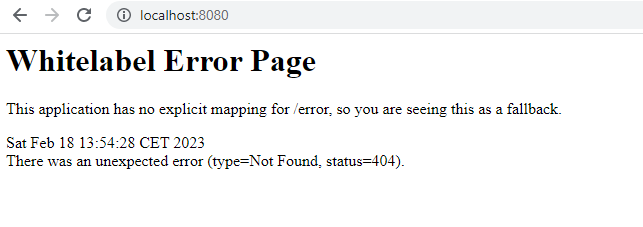
\includegraphics[width=\textwidth]{./images/chapter2/whitelabel_error_page.png}} 

Port 8080 is the default port. If this port is not available you will see an error message in Spring Boot's logging.

\begin{lstlisting}[frame=single]
***************************
APPLICATION FAILED TO START
***************************

Description:

Web server failed to start. Port 8080 was already in use.
\end{lstlisting}

The port number can be changed in the file application.properties. You have to add the property server.port here with the desired port number.

\begin{lstlisting}[frame=single]
server.port=8081
\end{lstlisting}

\subsection{Component}


\begin{lstlisting}
@Component
public class DependencyInjectionWithSpring implements CommandLineRunner {
   
   @Override    
   public void run(String... args) throws Exception {
	   System.out.println("Welcome to Java Advanced");
   }
}
\end{lstlisting}

De Spring Boot de CommandLineRunner interface voorziet de mogelijkheid om een stukje code uit te voeren zodra de Spring Boot applicatie ge\"initialiseerd is. 

Zodra je de CommandLineRunner interface implementeert in een klasse kan je de run-methode overschrijven. In de run-methode plaats je de code die uitgevoerd moet worden
als de applicatie opstart.  Zodra de Spring Boot applicatie opstart worden een aantal initialisatie-fasen doorlopen.  Eerst wordt de \textbf{application context} aangemaakt en alle Spring beans worden geladen. Als de applicatie volledige is ge\"initialiseerd wordt de run-methode van de CommandLineRunner automatisch door het Spring boot framework aangeroepen.



\subsubsection{Spring beans}

Spring Beans zijn componenten die volledig worden beheerd door het Spring Boot framework. Je hoeft zelf geen instanties van deze klassen te maken, Spring Boot genereert de objecten automatisch.  Daarnaast beheert Spring Boot ook de objecten. Wanneer een klasse gebruik wil maken van de functionaliteiten van een dergelijke Spring Bean, zal Spring Boot ervoor zorgen dat de instantie van de Spring Bean beschikbaar is voor de betreffende klasse.

\subsubsection{Application context}

De Application context is een belangrijk onderdeel van elke Spring Boot applicatie.
Hierin wordt namelijk bijgehouden welke infals een slimme doos waarin alle informatie en instellingen voor je Spring Boot-toepassing worden bewaard. Deze doos zorgt ervoor dat alle onderdelen van je applicatie met elkaar kunnen praten en weten waar ze moeten zoeken voor dingen zoals configuratie, gegevensbronnen en andere beans (componenten). Het maakt je Spring Boot-applicatie georganiseerd en helpt deze soepel te werken door alles op één plek te houden. Je kunt de application context beschouwen als het brein van je Spring Boot-applicatie dat alles coördineert en beschikbaar maakt voor de verschillende onderdelen van je programma.


Iets meer info tonen:

spring.application.name=My Demo

package be.pxl.demo.beans;

import org.springframework.boot.CommandLineRunner;
import org.springframework.context.ApplicationContext;
import org.springframework.stereotype.Component;

import java.time.LocalDateTime;
import java.time.ZoneId;
import java.time.ZoneOffset;

@Component
public class DependencyInjectionWithSpring implements CommandLineRunner {
	private final ApplicationContext applicationContext;

	public DependencyInjectionWithSpring(ApplicationContext applicationContext) {
		this.applicationContext = applicationContext;
	}

	@Override
   public void run(String... args) throws Exception {
	   System.out.println("Welcome to Java Advanced");
		System.out.println(applicationContext.getApplicationName());
		System.out.println(applicationContext.getDisplayName());
		System.out.println(applicationContext.getId());
		LocalDateTime dateTime = convertStartupDateToLocalDateTime(applicationContext.getStartupDate());
		System.out.println(dateTime);
		System.out.println(LocalDateTime.now());
   }


   private LocalDateTime convertStartupDateToLocalDateTime(long startupDate) {
	   // Get the system's default timezone
	   ZoneId systemZoneId = ZoneId.systemDefault();
	   // Get the ZoneOffset for the system's default timezone
	   ZoneOffset systemZoneOffset = systemZoneId.getRules().getOffset(LocalDateTime.now());
		return LocalDateTime.ofEpochSecond(applicationContext.getStartupDate() / 1000, 0, systemZoneOffset);

   }
}



Spring Boot Application Context:
When your Spring Boot application starts, it goes through various phases of initialization. After the application context is prepared and all beans are loaded, any classes implementing CommandLineRunner are executed.

\subsection{The Maven pom file}

POM stands for \'Project Object Model\'. It is an XML representation of a Maven project held in a file named pom.xml. This file can be found in your project directory. The POM contains all necessary information about a project, as well as configurations of plugins to be used during the build process. We will cover Maven in chapter 3.

\begin{lstlisting}[frame=single]
<?xml version="1.0" encoding="UTF-8"?>
<project xmlns="http://maven.apache.org/POM/4.0.0" xmlns:xsi="http://www.w3.org/2001/XMLSchema-instance"
         xsi:schemaLocation="http://maven.apache.org/POM/4.0.0 https://maven.apache.org/xsd/maven-4.0.0.xsd">
    <modelVersion>4.0.0</modelVersion>
    <parent>
        <groupId>org.springframework.boot</groupId>
        <artifactId>spring-boot-starter-parent</artifactId>
        <version>3.0.2</version>
        <relativePath/> <!-- lookup parent from repository -->
    </parent>
    <groupId>be.pxl</groupId>
    <artifactId>demo</artifactId>
    <version>0.0.1-SNAPSHOT</version>
    <name>demo</name>
    <description>demo</description>
    <properties>
        <java.version>17</java.version>
    </properties>
    <dependencies>
        <dependency>
            <groupId>org.springframework.boot</groupId>
            <artifactId>spring-boot-starter-web</artifactId>
        </dependency>

        <dependency>
            <groupId>org.springframework.boot</groupId>
            <artifactId>spring-boot-starter-test</artifactId>
            <scope>test</scope>
        </dependency>
    </dependencies>

    <build>
        <plugins>
            <plugin>
                <groupId>org.springframework.boot</groupId>
                <artifactId>spring-boot-maven-plugin</artifactId>
            </plugin>
        </plugins>
    </build>
</project>
\end{lstlisting}

spring-boot-starter-parent is a starter project that provides the default configuration for spring-based applications. Here you choose the version of Spring Boot.

For large projects, managing the dependencies is not always easy. Spring Boot solves this problem by grouping certain dependencies together. These groups of dependencies are called starters. All Spring Boot starters are named following the same naming pattern. The all start with spring-boot-starter-*, where * indicates the purpose and functionality provided by the starter.

spring-boot-starter-web adds all the libraries we need to develop web components. An embedded server will be provided in the Spring Boot project. Therefore the environment where the Spring Boot project is executed does not need to have a pre-installed server. The default embedded server for Spring Boot is Tomcat. The Spring MVC framework which provides all classes for developing RESTful web services is also part of spring-boot-starter-web.

spring-boot-starter-test (with scope test) is the starter for testing Spring Boot applications with libraries including JUnit Jupiter, Hamcrest and Mockito.

Inversion of Control (IoC) is \'e\'en van de basisprincipes van het Spring framework.
Bij Inversion of Control is het aanmaken en beheren van objecten niet langer de verantwoordelijkheid van de objecten zelf, maar is er een aparte 

So, Inversion of Control is about shifting the responsibility of managing object interactions from your code to a higher-level component (the framework or container). This makes your code more modular and flexible, as you rely on the framework to provide and coordinate the necessary components, 

To explain this in layman's terms, suppose you drive a car to your work place. This means you control the car. The IoC principle suggests to invert the control, meaning that instead of driving the car yourself, you hire a cab, where another person will drive the car.

What is a Bean in Spring Boot? A Bean is an object that is managed by the Spring framework. It is created, managed, and managed by the Spring container. Beans can be used to encapsulate and provide services, utilities, and functionalities to other components in an application.

In Spring, the objects that form the backbone of your application and that are managed by the Spring IoC container are called beans. A bean is an object that is instantiated, assembled, and otherwise managed by a Spring IoC container. Otherwise, a bean is simply one of many objects in your application.

TODO add image





IOC en dependency injection 


@Component
public class DependencyInjectionWithSpring implements CommandLineRunner {
   
   @Autowired
   private WeatherService weatherService;
   
   @Override    
   public void run(String... args) throws Exception {
	   weatherService.printWeather();
   }
}

WeatherService.java

import org.springframework.stereotype.Component;

@Component
public class WeatherService {
   public void printWeather() {
      System.out.println("The weather is sunny with a 20% chance of rain");
   }
}


Exercise

Create the class 





\subsection{@SpringBootApplication}

Java annotations are a mechanism for adding metadata information to our source code. An annotation processor processes these annotations at compile time or runtime to provide functionality such as code generation, error checking, etc.

@SpringBootApplication annotation is used to enable following three features:
\begin{itemize}
\item @EnableAutoConfiguration: enable Spring Boot’s auto-configuration mechanism
\item @ComponentScan: enable @Component scan on the package where the application is located
\item @Configuration: allow to register extra beans in the context or import additional configuration classes
\end{itemize}


\subsection{Auto-configuration}

Spring Boot auto-configuration attempts to automatically configure your Spring application based on the dependencies that you have added.
To gain some insight in this auto-configuration let's add a line in the application.properties file. This file can be found in the directory /src/main/resources. 

\begin{lstlisting}
logging.level.org.springframework=debug
\end{lstlisting}

logging.level.org.springframework is a application properties. A list of all available application properties can be found at \url{https://docs.spring.io/spring-boot/docs/current/reference/html/application-properties.html}.

\begin{oefening}
Add the line above to the application.properties file and restart the Spring Boot application.
\end{oefening}

In the console you will find all the auto-configuration Spring Boot is doing.